% Options for packages loaded elsewhere
\PassOptionsToPackage{unicode}{hyperref}
\PassOptionsToPackage{hyphens}{url}
\PassOptionsToPackage{dvipsnames,svgnames,x11names}{xcolor}
%
\documentclass[
]{report}

\usepackage{amsmath,amssymb}
\usepackage{lmodern}
\usepackage{iftex}
\ifPDFTeX
  \usepackage[T1]{fontenc}
  \usepackage[utf8]{inputenc}
  \usepackage{textcomp} % provide euro and other symbols
\else % if luatex or xetex
  \usepackage{unicode-math}
  \defaultfontfeatures{Scale=MatchLowercase}
  \defaultfontfeatures[\rmfamily]{Ligatures=TeX,Scale=1}
\fi
% Use upquote if available, for straight quotes in verbatim environments
\IfFileExists{upquote.sty}{\usepackage{upquote}}{}
\IfFileExists{microtype.sty}{% use microtype if available
  \usepackage[]{microtype}
  \UseMicrotypeSet[protrusion]{basicmath} % disable protrusion for tt fonts
}{}
\makeatletter
\@ifundefined{KOMAClassName}{% if non-KOMA class
  \IfFileExists{parskip.sty}{%
    \usepackage{parskip}
  }{% else
    \setlength{\parindent}{0pt}
    \setlength{\parskip}{6pt plus 2pt minus 1pt}}
}{% if KOMA class
  \KOMAoptions{parskip=half}}
\makeatother
\usepackage{xcolor}
\setlength{\emergencystretch}{3em} % prevent overfull lines
\setcounter{secnumdepth}{5}
% Make \paragraph and \subparagraph free-standing
\ifx\paragraph\undefined\else
  \let\oldparagraph\paragraph
  \renewcommand{\paragraph}[1]{\oldparagraph{#1}\mbox{}}
\fi
\ifx\subparagraph\undefined\else
  \let\oldsubparagraph\subparagraph
  \renewcommand{\subparagraph}[1]{\oldsubparagraph{#1}\mbox{}}
\fi


\providecommand{\tightlist}{%
  \setlength{\itemsep}{0pt}\setlength{\parskip}{0pt}}\usepackage{longtable,booktabs,array}
\usepackage{calc} % for calculating minipage widths
% Correct order of tables after \paragraph or \subparagraph
\usepackage{etoolbox}
\makeatletter
\patchcmd\longtable{\par}{\if@noskipsec\mbox{}\fi\par}{}{}
\makeatother
% Allow footnotes in longtable head/foot
\IfFileExists{footnotehyper.sty}{\usepackage{footnotehyper}}{\usepackage{footnote}}
\makesavenoteenv{longtable}
\usepackage{graphicx}
\makeatletter
\def\maxwidth{\ifdim\Gin@nat@width>\linewidth\linewidth\else\Gin@nat@width\fi}
\def\maxheight{\ifdim\Gin@nat@height>\textheight\textheight\else\Gin@nat@height\fi}
\makeatother
% Scale images if necessary, so that they will not overflow the page
% margins by default, and it is still possible to overwrite the defaults
% using explicit options in \includegraphics[width, height, ...]{}
\setkeys{Gin}{width=\maxwidth,height=\maxheight,keepaspectratio}
% Set default figure placement to htbp
\makeatletter
\def\fps@figure{htbp}
\makeatother

\usepackage{pdftexcmds}
\makeatletter
\let\pdfstrcmp\pdf@strcmp
\let\pdffilemoddate\pdf@filemoddate
\makeatother
\usepackage[inkscape={/usr/bin/inkscape}]{svg}
\usepackage{svg}
\makeatletter
\@ifpackageloaded{tcolorbox}{}{\usepackage[many]{tcolorbox}}
\@ifpackageloaded{fontawesome5}{}{\usepackage{fontawesome5}}
\definecolor{quarto-callout-color}{HTML}{909090}
\definecolor{quarto-callout-note-color}{HTML}{0758E5}
\definecolor{quarto-callout-important-color}{HTML}{CC1914}
\definecolor{quarto-callout-warning-color}{HTML}{EB9113}
\definecolor{quarto-callout-tip-color}{HTML}{00A047}
\definecolor{quarto-callout-caution-color}{HTML}{FC5300}
\definecolor{quarto-callout-color-frame}{HTML}{acacac}
\definecolor{quarto-callout-note-color-frame}{HTML}{4582ec}
\definecolor{quarto-callout-important-color-frame}{HTML}{d9534f}
\definecolor{quarto-callout-warning-color-frame}{HTML}{f0ad4e}
\definecolor{quarto-callout-tip-color-frame}{HTML}{02b875}
\definecolor{quarto-callout-caution-color-frame}{HTML}{fd7e14}
\makeatother
\makeatletter
\makeatother
\makeatletter
\makeatother
\makeatletter
\@ifpackageloaded{caption}{}{\usepackage{caption}}
\AtBeginDocument{%
\ifdefined\contentsname
  \renewcommand*\contentsname{Table of contents}
\else
  \newcommand\contentsname{Table of contents}
\fi
\ifdefined\listfigurename
  \renewcommand*\listfigurename{List of Figures}
\else
  \newcommand\listfigurename{List of Figures}
\fi
\ifdefined\listtablename
  \renewcommand*\listtablename{List of Tables}
\else
  \newcommand\listtablename{List of Tables}
\fi
\ifdefined\figurename
  \renewcommand*\figurename{Figure}
\else
  \newcommand\figurename{Figure}
\fi
\ifdefined\tablename
  \renewcommand*\tablename{Table}
\else
  \newcommand\tablename{Table}
\fi
}
\@ifpackageloaded{float}{}{\usepackage{float}}
\floatstyle{ruled}
\@ifundefined{c@chapter}{\newfloat{codelisting}{h}{lop}}{\newfloat{codelisting}{h}{lop}[chapter]}
\floatname{codelisting}{Listing}
\newcommand*\listoflistings{\listof{codelisting}{List of Listings}}
\makeatother
\makeatletter
\@ifpackageloaded{caption}{}{\usepackage{caption}}
\@ifpackageloaded{subcaption}{}{\usepackage{subcaption}}
\makeatother
\makeatletter
\@ifpackageloaded{tcolorbox}{}{\usepackage[many]{tcolorbox}}
\makeatother
\makeatletter
\@ifundefined{shadecolor}{\definecolor{shadecolor}{rgb}{.97, .97, .97}}
\makeatother
\makeatletter
\makeatother
\ifLuaTeX
  \usepackage{selnolig}  % disable illegal ligatures
\fi
\IfFileExists{bookmark.sty}{\usepackage{bookmark}}{\usepackage{hyperref}}
\IfFileExists{xurl.sty}{\usepackage{xurl}}{} % add URL line breaks if available
\urlstyle{same} % disable monospaced font for URLs
\hypersetup{
  pdftitle={Robust Passivity-Based Control},
  colorlinks=true,
  linkcolor={blue},
  filecolor={Maroon},
  citecolor={Blue},
  urlcolor={Blue},
  pdfcreator={LaTeX via pandoc}}

\title{Robust Passivity-Based Control}
\author{}
\date{}

\begin{document}
\maketitle
\ifdefined\Shaded\renewenvironment{Shaded}{\begin{tcolorbox}[sharp corners, interior hidden, frame hidden, boxrule=0pt, breakable, borderline west={3pt}{0pt}{shadecolor}, enhanced]}{\end{tcolorbox}}\fi

\renewcommand*\contentsname{Table of contents}
{
\hypersetup{linkcolor=}
\setcounter{tocdepth}{2}
\tableofcontents
}
\hypertarget{robust-passivity-based-control-of-underactuated-systems-via-neural-approximators-and-bayesian-inference}{%
\section{Robust Passivity-Based Control of Underactuated Systems via
Neural Approximators and Bayesian
Inference}\label{robust-passivity-based-control-of-underactuated-systems-via-neural-approximators-and-bayesian-inference}}

Boise State University

\textbf{Authors}: Nardos Ayele Ashenafi           ~ Wankun
Sirichotiyakul, Ph.D.~           ~ Aykut C. Satici, Ph.D.~

\hypertarget{underactuated-robots}{%
\section{Underactuated Robots}\label{underactuated-robots}}

\begin{figure}

\begin{minipage}[t]{0.50\linewidth}

{\centering 

\includegraphics{contents/assets/manipulator.jpg} Torque-limited
manipulators

}

\end{minipage}%
%
\begin{minipage}[t]{0.50\linewidth}

{\centering 

~ \includegraphics{contents/assets/underactuation-illustration.png} ~
Walking robots

}

\end{minipage}%

\end{figure}

\hypertarget{existing-methods}{%
\section{Existing Methods}\label{existing-methods}}

\begin{figure}

\begin{minipage}[c]{0.61\linewidth}

{\centering 

\textbf{Passivity-based Control}
\includegraphics{contents/assets/pbc-outline.svg}

}

\end{minipage}%
%
\begin{minipage}[c]{0.03\linewidth}

{\centering 

~

}

\end{minipage}%
%
\begin{minipage}[c]{0.36\linewidth}

{\centering 

\begin{description}
\tightlist
\item[Strengths]
Stability guarantees\\
Closed-form policy
\item[Weaknesses]
Model uncertainties\\
Need to solve PDEs
\end{description}

}

\end{minipage}%

\end{figure}

\begin{figure}

\begin{minipage}[c]{0.61\linewidth}

{\centering 

\textbf{Reinforcement learning}
\includegraphics{contents/assets/rl-outline.svg}

}

\end{minipage}%
%
\begin{minipage}[c]{0.03\linewidth}

{\centering 

~

}

\end{minipage}%
%
\begin{minipage}[c]{0.36\linewidth}

{\centering 

\begin{description}
\tightlist
\item[Strengths]
More general\\
Unknown dynamics OK
\item[Weaknesses]
Sample complexity\\
Stability guarantees?
\end{description}

}

\end{minipage}%

\end{figure}

\hypertarget{data-driven-passivity-based-control}{%
\section{Data-Driven Passivity-Based
Control}\label{data-driven-passivity-based-control}}

\begin{figure}

\begin{minipage}[c]{0.61\linewidth}

{\centering 

\includegraphics{contents/assets/pbc-outline-cross.svg}

}

\end{minipage}%
%
\begin{minipage}[c]{0.03\linewidth}

{\centering 

~

}

\end{minipage}%
%
\begin{minipage}[c]{0.36\linewidth}

{\centering 

~

}

\end{minipage}%

\end{figure}

\begin{figure}

\begin{minipage}[c]{0.61\linewidth}

{\centering 

\includegraphics{contents/assets/pbc-ml-outline.svg}

}

\end{minipage}%
%
\begin{minipage}[c]{0.03\linewidth}

{\centering 

~

}

\end{minipage}%
%
\begin{minipage}[c]{0.36\linewidth}

{\centering 

\begin{itemize}
\tightlist
\item
  Systematic approach
\item
  Prior domain knowledge
\item
  Stability is \emph{intrinsic}
\item
  Model uncertainty considerations via Bayesian learning
\end{itemize}

}

\end{minipage}%

\end{figure}

\hypertarget{background}{%
\chapter{Background}\label{background}}

Passive System Theory and Passivity-Based Control (PBC)

\hypertarget{passivity}{%
\section{Passivity}\label{passivity}}

A dynamical system

\[
\Sigma: \quad
\begin{cases}
  \dot{x} &= f(x,u) \\
  y &= h(x,u)
\end{cases}
\quad x \in \mathcal{X} \subset \mathbb{R}^{2n}, \, u \in \mathcal{U} \subset \mathbb{R}^{m} 
\]

is \textbf{dissipative} with respect to some supply rate \(s\) if there
exists a \emph{storage function}
\(\mathcal{H}: \mathcal{X} \to \mathbb{R}^{+}\) such that

\[
\mathcal{H}\left(  x(t_1) \right) \leq  \mathcal{H}\left(  x(t_0) \right) + \int_{t_0}^{t_1} s(u(t), y(t)) \, \text{d}t
\]

for all \(x(t_0) = x_0\), all input \(u\), and all \(t_1 \geq t_0\)

The system \(\Sigma\) is \textbf{passive} if it is dissipative with
supply rate

\[s = u^\top y.\]

\hypertarget{passive-system-example}{%
\section{Passive System Example}\label{passive-system-example}}

\includegraphics{contents/assets/passive-system-example.png}

Kirchoff's law

\[
\begin{aligned}
v &= Ri + \frac{1}{C} \int_{0}^{t} i(\tau) \, \text{d}\tau + L \frac{\text{d} i}{\text{d} t} \\
vi - Ri^2 &= \frac{\text{d}}{\text{d} t} \left( 
  \underbrace{\frac{1}{2C} \left( \int_{0}^{t} i(\tau)\, \text{d} \tau \right)^2}_{\mathcal{V}} + 
  \underbrace{\frac{1}{2} Li^2}_{\mathcal{T}}  
\right)
\end{aligned}
\]

Let \(\mathcal{H} = \mathcal{V} + \mathcal{T}\), integrate to obtain

\[
\underbrace{\mathcal{H}(t)}_{\textrm{available}} -
\underbrace{\mathcal{H}(0)}_{\textrm{initial}} 
= 
\underbrace{\int_{0}^{t} v(\tau)i(\tau)\, \text{d} \tau}_{\textrm{supplied}} - 
\underbrace{\int_{0}^{t} Ri^2(\tau)\, \text{d} \tau}_{\textrm{dissipated}}
<
\int_{0}^{t} v(\tau) i(\tau) \, \text{d} \tau
\]

\hypertarget{stability-of-passive-systems}{%
\section{Stability of Passive
Systems}\label{stability-of-passive-systems}}

\[
\Sigma: \quad
\begin{cases}
  \dot{x} &= f(x,u), && f(0,0) = 0, \\
  y &= h(x,u), && h(0,0) = 0,
\end{cases}
\]

\begin{tcolorbox}[enhanced jigsaw, opacityback=0, breakable, leftrule=.75mm, toptitle=1mm, rightrule=.15mm, toprule=.15mm, bottomrule=.15mm, opacitybacktitle=0.6, colbacktitle=quarto-callout-note-color!10!white, colframe=quarto-callout-note-color-frame, title={Lemma (Khalil, 2002)}, bottomtitle=1mm, left=2mm, colback=white, arc=.35mm, titlerule=0mm, coltitle=black]
The origin of \(\Sigma\) is \emph{stable}, i.e \[
y \equiv 0 \implies x \equiv 0
\] if \(\Sigma\) is passive, i.e \[
\mathcal{H} \geq 0,\quad \dot{\mathcal{H}} = \frac{\partial\mathcal{H}}{\partial x} f(x,u) \leq u^{\top} y 
\]
\end{tcolorbox}

\hypertarget{passivity-based-control-pbc}{%
\section{Passivity-Based Control
(PBC)}\label{passivity-based-control-pbc}}

\[
\Sigma_o: \quad
\begin{cases}
  \dot{x} &= f(x) + g(x)u, \\
  y &= h(x)
\end{cases}
\]

Main idea --- Select \(u(x) = u_{es} + u_{di}\) that renders the
closed-loop system passive.

\[
\Sigma_d: \quad
\begin{cases}
  \dot{x} &= f_d(x) + g(x) u_{di}, \quad f_d := f(x) + g(x) u_{es}(x) \\
  y_d &= h_d(x)
\end{cases}
\]

Control problem is cast as a search for \(H_d\) and \(h_d\) s.t.
\(\dot{H}_d \leq y_d^\top u_{di}\)

\hypertarget{pbc-example---simple-pendulum}{%
\section{PBC Example - Simple
Pendulum}\label{pbc-example---simple-pendulum}}

\begin{tcolorbox}[enhanced jigsaw, opacityback=0, breakable, leftrule=.75mm, toptitle=1mm, rightrule=.15mm, toprule=.15mm, bottomrule=.15mm, opacitybacktitle=0.6, colbacktitle=quarto-callout-note-color!10!white, colframe=quarto-callout-note-color-frame, title={System Dynamics}, bottomtitle=1mm, left=2mm, colback=white, arc=.35mm, titlerule=0mm, coltitle=black]

\(H(q,p) = \frac{1}{2} J^{-1} p^2 + mgl (1 - \cos q)\)

\[
\begin{bmatrix} \dot{q} \\ \dot{p} \end{bmatrix} = 
\begin{bmatrix} \phantom{-}0 & 1 \\ -1 & 0 \end{bmatrix} 
\begin{bmatrix} \nabla_q H_{\phantom{d}} \\ \nabla_p H_{\phantom{d}} \end{bmatrix} +
\begin{bmatrix} 0 \\ G \end{bmatrix} u_\phantom{di},
\qquad y = \dot{q}
\]

Choose \(u = u_{es} + u_{di}\) that transforms system into a passive one
with \(x^\star = (q^\star, 0)\)

\(Gu_{es} = \nabla_q H - \nabla_q H_d , \quad Gu_{di} = -GK_D G^\top \nabla_p H_d\)

\[
\begin{bmatrix} \dot{q} \\ \dot{p} \end{bmatrix} = 
\begin{bmatrix} \phantom{-}0 & 1 \\ -1 & 0 \end{bmatrix} 
\begin{bmatrix} \nabla_q H_d \\ \nabla_p H_d \end{bmatrix} +
\begin{bmatrix} 0 \\ G \end{bmatrix} u_{di},
\qquad y = \dot{q}
\]

\[
\begin{bmatrix} \dot{q} \\ \dot{p} \end{bmatrix} = 
\begin{bmatrix} \phantom{-}0 & 1 \\ -1 & -G K_D G^\top \end{bmatrix} 
\begin{bmatrix} \nabla_q H_d \\ \nabla_p H_d \end{bmatrix},
\qquad y = \dot{q}
\]

\end{tcolorbox}

\hypertarget{pbc-example---simple-pendulum-1}{%
\section{PBC Example - Simple
Pendulum}\label{pbc-example---simple-pendulum-1}}

\begin{tcolorbox}[enhanced jigsaw, opacityback=0, breakable, leftrule=.75mm, toptitle=1mm, rightrule=.15mm, toprule=.15mm, bottomrule=.15mm, opacitybacktitle=0.6, colbacktitle=quarto-callout-tip-color!10!white, colframe=quarto-callout-tip-color-frame, title={Control Synthesis via PBC}, bottomtitle=1mm, left=2mm, colback=white, arc=.35mm, titlerule=0mm, coltitle=black]

Choose \(u = u_{es} + u_{di}\) that transforms system into a passive one
with \(x^\star = (q^\star, 0)\)

\(Gu_{es} = \nabla_q H - \nabla_q H_d , \quad Gu_{di} = -GK_D G^\top \nabla_p H_d\)

\[
\begin{bmatrix} \dot{q} \\ \dot{p} \end{bmatrix} = 
\begin{bmatrix} \phantom{-}0 & 1 \\ -1 & -G K_D G^\top \end{bmatrix} 
\begin{bmatrix} \nabla_q H_d \\ \nabla_p H_d \end{bmatrix},
\qquad y = \dot{q}
\]

\(H_d(q,p) = \frac{1}{2} J^{-1} p^2 + V_d(q), \quad V_d(q) = \frac{1}{2} K_{P} \left( q - q^\star \right)^2\)

\(\dot{H}_d = -K_D \left( J^{-1} p \right)^2 = y^\top u_{di} \leq 0\)

\(\boxed{u = -mgl\sin(x) - K_P(q - q^\star) - K_D \dot{q}}\)

\end{tcolorbox}

\hypertarget{high-dimensional-problem-ballbot}{%
\section{High-dimensional Problem:
Ballbot}\label{high-dimensional-problem-ballbot}}

\includegraphics[width=\textwidth,height=6.66667in]{contents/assets/Ballbot_Rezero_2010.jpg}

\includegraphics[width=8.33333in,height=\textheight]{contents/assets/ballbot_schematic.png}

\includegraphics[width=8.33333in,height=\textheight]{contents/assets/ballbot_derivation_1.png}

\includegraphics[width=8.33333in,height=\textheight]{contents/assets/ballbot_derivation_2.png}

\hypertarget{our-methods}{%
\section{Our Methods}\label{our-methods}}

\begin{figure}

\begin{minipage}[c]{0.10\linewidth}

{\centering 

~

}

\end{minipage}%
%
\begin{minipage}[c]{0.80\linewidth}

{\centering 

\includegraphics{contents/assets/pbc-ml-outline.svg}

}

\end{minipage}%
%
\begin{minipage}[c]{0.10\linewidth}

{\centering 

~

}

\end{minipage}%

\end{figure}

\begin{tcolorbox}[enhanced jigsaw, opacityback=0, breakable, leftrule=.75mm, toptitle=1mm, rightrule=.15mm, toprule=.15mm, bottomrule=.15mm, opacitybacktitle=0.6, colbacktitle=quarto-callout-note-color!10!white, colframe=quarto-callout-note-color-frame, title={Data-Driven Passivity-based control}, bottomtitle=1mm, left=2mm, colback=white, arc=.35mm, titlerule=0mm, coltitle=black]
\[
\begin{aligned}
\underset{\theta}{\text{minimize}} && J(\theta, x_0) &= \int_{0}^{T} \ell \left(\phi,u^\theta,\theta\right)\, \text{d} t \\
\text{subject to} &&
\begin{bmatrix}
  \dot{q} \\ \dot{p}
\end{bmatrix} &=
\begin{bmatrix}
  0 & I \\ -I & 0
\end{bmatrix}
\begin{bmatrix} \nabla_q H \\ \nabla_p H \end{bmatrix} + 
\begin{bmatrix}
  0 \\ G
\end{bmatrix} u^{\theta}
\\
&& u^\theta &= -G^{\dagger} \nabla_q H_d^{\theta}  - K_D G^\top \nabla_p H_d^{\theta}
\end{aligned}
\]
\end{tcolorbox}

\hypertarget{neuralpbc-problem-statement}{%
\section{\texorpdfstring{\textsc{NeuralPbc} Problem
Statement}{NeuralPbc Problem Statement}}\label{neuralpbc-problem-statement}}

\begin{tcolorbox}[enhanced jigsaw, opacityback=0, breakable, leftrule=.75mm, toptitle=1mm, rightrule=.15mm, toprule=.15mm, bottomrule=.15mm, opacitybacktitle=0.6, colbacktitle=quarto-callout-note-color!10!white, colframe=quarto-callout-note-color-frame, title={Data-Driven Passivity-based control}, bottomtitle=1mm, left=2mm, colback=white, arc=.35mm, titlerule=0mm, coltitle=black]
\[
\begin{aligned}
\underset{\theta}{\text{minimize}} && J(\theta, x_0) &= \int_{0}^{T} \ell \left(\phi,u^\theta,\theta\right)\, \text{d} t \\
\text{subject to} &&
\begin{bmatrix}
  \dot{q} \\ \dot{p}
\end{bmatrix} &=
\begin{bmatrix}
  0 & I \\ -I & 0
\end{bmatrix}
\begin{bmatrix} \nabla_q H \\ \nabla_p H \end{bmatrix} + 
\begin{bmatrix}
  0 \\ G
\end{bmatrix} u^{\theta}
\\
&& u^\theta &= -G^{\dagger} \nabla_q H_d^{\theta}  - K_D G^\top \nabla_p H_d^{\theta}
\end{aligned}
\]
\end{tcolorbox}

\begin{itemize}
\tightlist
\item
  Sampling the state space efficiently
\item
  Injecting control task into loss function design
\item
  Backprop through closed-loop trajectories
\end{itemize}

\hypertarget{neuralpbc-sampling-state-space}{%
\section{\texorpdfstring{\textsc{NeuralPbc} Sampling State Space
{📉}}{NeuralPbc Sampling State Space 📉}}\label{neuralpbc-sampling-state-space}}

\includegraphics{contents/assets/neuralpbc/000.svg}

\includegraphics{contents/assets/neuralpbc/001.svg}

\includegraphics{contents/assets/neuralpbc/002.svg}

\includegraphics{contents/assets/neuralpbc/003.svg}

\includegraphics{contents/assets/neuralpbc/004.svg}

\includegraphics{contents/assets/neuralpbc/005.svg}

\includegraphics{contents/assets/neuralpbc/006.svg}

\includegraphics{contents/assets/neuralpbc/007.svg}

\includegraphics{contents/assets/neuralpbc/008.svg}

\includegraphics{contents/assets/neuralpbc/009.svg}

\includegraphics{contents/assets/neuralpbc/010.svg}

\includegraphics{contents/assets/neuralpbc/011.svg}

\includegraphics{contents/assets/neuralpbc/012.svg}

\includegraphics{contents/assets/neuralpbc/013.svg}

\includegraphics{contents/assets/neuralpbc/014.svg}

\includegraphics{contents/assets/neuralpbc/016.svg}

\includegraphics{contents/assets/neuralpbc/017.svg}

\includegraphics{contents/assets/neuralpbc/018.svg}

\includegraphics{contents/assets/neuralpbc/019.svg}

\includegraphics{contents/assets/neuralpbc/020.svg}

\includegraphics{contents/assets/neuralpbc/021.svg}

\includegraphics{contents/assets/neuralpbc/022.svg}

\includegraphics{contents/assets/neuralpbc/023.svg}

\includegraphics{contents/assets/neuralpbc/024.svg}

\includegraphics{contents/assets/neuralpbc/025.svg}

\includegraphics{contents/assets/neuralpbc/026.svg}

\includegraphics{contents/assets/neuralpbc/027.svg}

\includegraphics{contents/assets/neuralpbc/028.svg}

\includegraphics{contents/assets/neuralpbc/029.svg}

\includegraphics{contents/assets/neuralpbc/030.svg}

\includegraphics{contents/assets/neuralpbc/031.svg}

\includegraphics{contents/assets/neuralpbc/032.svg}

\includegraphics{contents/assets/neuralpbc/033.svg}

\hypertarget{neuralpbc-cost-function}{%
\section{\texorpdfstring{\textsc{NeuralPbc} Cost
Function}{NeuralPbc Cost Function}}\label{neuralpbc-cost-function}}

\[
J(\theta, x_0) = \int_{0}^{T} \ell \left(\phi,u^\theta,\theta\right)\, \text{d} t
\]

\(\ell \triangleq \ell_{\text{set}}(\gamma) + \ell_{\bot}(\gamma,u)\)
where

\begin{itemize}
\item
  \(\phi\) is the flow of the equation of motion
\item
  \(\gamma\) is the closed-loop trajectory starting from \(x_0\)
\item
  \(T\) is the time horizon (hyperparameter)
\end{itemize}

\hypertarget{neuralpbc-cost-function-1}{%
\section{\texorpdfstring{\textsc{NeuralPbc} Cost
Function}{NeuralPbc Cost Function}}\label{neuralpbc-cost-function-1}}

\[\ell \triangleq \ell_{\text{set}}(\gamma) + \ell_{\bot}(\gamma,u)\]

\begin{tcolorbox}[enhanced jigsaw, bottomrule=.15mm, arc=.35mm, colframe=quarto-callout-color-frame, breakable, leftrule=.75mm, rightrule=.15mm, colback=white, toprule=.15mm, left=2mm, opacityback=0]

Penalizes when closed-loop trajectory \(\gamma\) under the current
control law is far away from a neighborhood \(\mathcal{S}\) of
\(x^\star\)

\begin{figure}

\begin{minipage}[t]{0.50\linewidth}

{\centering 

\includegraphics{contents/assets/pend_damped_phase_edited.svg}

}

\end{minipage}%
%
\begin{minipage}[t]{0.50\linewidth}

{\centering 

\[
\ell_{\text{set}}(x) = \underset{t}{\inf} \left\{ \lVert a-b \rVert : a \in \gamma(t), b \in \mathcal{S}\right\}
\]

\begin{itemize}
\tightlist
\item
  The set \(\mathcal{S}\) may be chosen as

  \begin{itemize}
  \tightlist
  \item
    A ball around \(x^\star\)
  \item
    Estimated region of attraction
  \end{itemize}
\item
  No additional loss if any point in \(\gamma\) is in \(\mathcal{S}\)
\end{itemize}

}

\end{minipage}%

\end{figure}

\end{tcolorbox}

\hypertarget{neuralpbc-cost-function-2}{%
\section{\texorpdfstring{\textsc{NeuralPbc} Cost
Function}{NeuralPbc Cost Function}}\label{neuralpbc-cost-function-2}}

\[\ell \triangleq \ell_{\text{set}}(\gamma) + \ell_{\bot}(\gamma,u)\]

\begin{tcolorbox}[enhanced jigsaw, bottomrule=.15mm, arc=.35mm, colframe=quarto-callout-color-frame, breakable, leftrule=.75mm, rightrule=.15mm, colback=white, toprule=.15mm, left=2mm, opacityback=0]

Measures how close \(\gamma\) is to \(\gamma^\star\) (expert trajectory)
using transverse coordinates \(x_\bot\)

\begin{figure}

\begin{minipage}[t]{0.41\linewidth}

{\centering 

\raisebox{-\height}{

\includegraphics{contents/assets/transverseCoordinates.svg}

}

}

\end{minipage}%
%
\begin{minipage}[t]{0.59\linewidth}

{\centering 

\begin{itemize}
\tightlist
\item
  Coordinate transformation

  \begin{itemize}
  \tightlist
  \item
    \(\tau \in \mathbb{R}\) a surrogate for time
  \item
    \(x_{\bot} \in \mathbb{R}^{2n-1}\) quantify how far away the current
    state is from \(\gamma^\star\)
  \end{itemize}
\item
  By construction \(x_{\bot} \to 0 \iff \gamma = \gamma^\star\)
\end{itemize}

\[\ell_{\bot} = x_\bot^\top Q x_\bot + u^\top R u, \, Q \succeq 0, \, R \succ 0\]

\begin{itemize}
\tightlist
\item
  No preferred orbit? \(Q = 0\)
\end{itemize}

}

\end{minipage}%

\end{figure}

\end{tcolorbox}

\begin{itemize}
\tightlist
\item
  We can find a coordinate transformation such that 1 coordinate
  \(\tau\) is along the desired orbit and acts as surrogate for time
\item
  The remaining coordinates \(x_{\bot}\) quantify how far away the
  current state is from the desired trajectory
\end{itemize}

\hypertarget{backprop-through-ode-solutions}{%
\section{Backprop through ODE
Solutions}\label{backprop-through-ode-solutions}}

We need \(\partial J / \partial \theta\), which depends ODE solutions

{😿} Combining \texttt{autodiff} with numerical ODE solvers

{😿} Adjoint sensitivity method: solve the adjoint problem backward in
time
\[\frac{\text{d}\lambda}{\text{d}t} = -\lambda \frac{\partial f}{\partial x}, \quad \frac{\partial J}{\partial \theta} = \lambda(t_0) \frac{\partial f}{\partial x}\]

{😺} Adjoint methods + \texttt{autodiff} implemented in
\texttt{DiffEqFlux.jl}

\begin{itemize}
\tightlist
\item
  Plain \texttt{autodiff} causes errors due to numerical ODE
  integration, high memory consumption
\item
  Adjoint methods requires storing many passes of the adjoint problem,
  again high memory consumption
\item
  \texttt{DiffEqFlux} combines the two, avoiding multiple passes through
  clever implementation, fast an efficient
\end{itemize}

\hypertarget{robust-control-under-uncertainties}{%
\section{Robust Control Under
Uncertainties}\label{robust-control-under-uncertainties}}

\begin{tcolorbox}[enhanced jigsaw, opacityback=0, breakable, leftrule=.75mm, toptitle=1mm, rightrule=.15mm, toprule=.15mm, bottomrule=.15mm, opacitybacktitle=0.6, colbacktitle=quarto-callout-important-color!10!white, colframe=quarto-callout-important-color-frame, title={Optimal Control under System Parameter Uncertainties}, bottomtitle=1mm, left=2mm, colback=white, arc=.35mm, titlerule=0mm, coltitle=black]
\[
\begin{aligned}
\underset{\theta}{\text{minimize}} && J(\theta, x_0) &= \int_{0}^{T} \ell \left(\phi,u^\theta,\theta\right)\, \text{d} t \\
\text{subject to} &&
\dot{x} &= f(x, u^{\theta}; p)\\
&& p &\sim \, \mathcal{N}(\hat{p}, \sigma_p)
\end{aligned}
\]
\end{tcolorbox}

\begin{tcolorbox}[enhanced jigsaw, opacityback=0, breakable, leftrule=.75mm, toptitle=1mm, rightrule=.15mm, toprule=.15mm, bottomrule=.15mm, opacitybacktitle=0.6, colbacktitle=quarto-callout-important-color!10!white, colframe=quarto-callout-important-color-frame, title={Optimal Control under System Parameter and Measurement Uncertainties}, bottomtitle=1mm, left=2mm, colback=white, arc=.35mm, titlerule=0mm, coltitle=black]
\[
\begin{aligned}
\underset{\theta}{\text{minimize}} && J(\theta, x_0) &= \int_{0}^{T} \ell \left(\phi,u^\theta,\theta\right)\, \text{d} t \\
\text{subject to} &&
\dd x &= f(x, u^{\theta}) 
        \dd t + \nabla_x u(x) \dd W_t \\
&& p &\sim \,\mathcal{N}(\hat{p}, \sigma_p)
\end{aligned}
\]
\end{tcolorbox}

\includegraphics[width=6.25in,height=5.20833in]{contents/assets/regular_vs_bayesian.svg}

~

\begin{itemize}
\tightlist
\item
  BNNs capture variance in controller
\item
  Akin to learning ensemble of controllers that each minimize \(J\)
\end{itemize}

\hypertarget{bayesian-learning}{%
\section{Bayesian Learning}\label{bayesian-learning}}

\begin{tcolorbox}[enhanced jigsaw, opacityback=0, breakable, leftrule=.75mm, toptitle=1mm, rightrule=.15mm, toprule=.15mm, bottomrule=.15mm, opacitybacktitle=0.6, colbacktitle=quarto-callout-important-color!10!white, colframe=quarto-callout-important-color-frame, title={Bayesian Passivity-based Control}, bottomtitle=1mm, left=2mm, colback=white, arc=.35mm, titlerule=0mm, coltitle=black]
\[
\begin{aligned}
\underset{z}{\text{minimize}} && J(\theta, x_0) &= \int_{0}^{T} \ell \left(\phi,u^\theta,\theta\right)\, \text{d} t \\
\text{subject to} &&
\dd x &= f(x, u^{\theta}) 
        \dd t + \nabla_x u(x) \dd W_t \\
&& p &\sim \, \mathcal{N}(\hat{p}, \sigma_p) \\
&& u^\theta &= -G^{\dagger} \nabla_q H_d^{\theta}  - K_D G^\top \nabla_p H_d^{\theta} \\
&& \theta &\sim \, q(\theta; z)
\end{aligned}
\]
\end{tcolorbox}

~ \[
p(\theta \mid \mathcal{D}) = \frac{\overbrace{p(\mathcal{D} \mid
\theta)}^{\text{likelihood}}\overbrace{p(\theta)}^{\text{prior}}}
{\underbrace{\int_\theta p(\mathcal{D} \mid \theta^\prime)p(\theta^\prime)
d\theta^\prime}_{\text{evidence}}} \underbrace{\approx q(\theta;
z)}_{\text{VI}}.
\]

\begin{tcolorbox}[enhanced jigsaw, opacityback=0, breakable, leftrule=.75mm, toptitle=1mm, rightrule=.15mm, toprule=.15mm, bottomrule=.15mm, opacitybacktitle=0.6, colbacktitle=quarto-callout-important-color!10!white, colframe=quarto-callout-important-color-frame, title={KL-divergence and ELBO}, bottomtitle=1mm, left=2mm, colback=white, arc=.35mm, titlerule=0mm, coltitle=black]
\[
\begin{aligned}
D_{\text{KL}} &= \mathbb{E}_{\theta \sim q}\left[ \log \frac{q(\theta;
z)}{p(\theta \mid \mathcal{D})}\right] \\
&= \log p(\mathcal{D}) - \mathbb{E}_{\theta \sim q}\left[ \log
\frac{p(\mathcal{D} \mid \theta) p(\theta)}{q(\theta; z)} \right] \\
\mathcal{L}(\mathcal{D}; z) &= \mathbb{E}_{\theta \sim q}\left[ \log
p(\mathcal{D} \mid \theta) p(\theta) - \log q(\theta; z) \right]
\end{aligned}
\]
\end{tcolorbox}

\hypertarget{bayesian-solution}{%
\section{Bayesian Solution}\label{bayesian-solution}}

~

Computing ELBO
\[ \mathcal{L}(\mathcal{D};z) = \mathbb{E}_{\theta \sim q}\left[ \log p(\mathcal{D} \mid \theta)p(\theta) - \log q(\theta; z)  \right] \]
requires:

\begin{itemize}
\tightlist
\item
  \emph{Likelihood}:
\end{itemize}

\[ p( J(\theta, x_0)) = \mathcal{N}(0, s). 
\]

\begin{itemize}
\tightlist
\item
  \emph{Prior}:

  Uninformed

  Deterministic
\end{itemize}

\begin{tcolorbox}[enhanced jigsaw, opacityback=0, breakable, leftrule=.75mm, toptitle=1mm, rightrule=.15mm, toprule=.15mm, bottomrule=.15mm, opacitybacktitle=0.6, colbacktitle=quarto-callout-tip-color!10!white, colframe=quarto-callout-tip-color-frame, title={Prediction through maximum aposteriori}, bottomtitle=1mm, left=2mm, colback=white, arc=.35mm, titlerule=0mm, coltitle=black]
\[
u(x) = u(x, \underset{\theta}{\text{argmax}} \, p(\theta;z)).
\]
\end{tcolorbox}

\begin{tcolorbox}[enhanced jigsaw, opacityback=0, breakable, leftrule=.75mm, toptitle=1mm, rightrule=.15mm, toprule=.15mm, bottomrule=.15mm, opacitybacktitle=0.6, colbacktitle=quarto-callout-tip-color!10!white, colframe=quarto-callout-tip-color-frame, title={Prediction through marginalization}, bottomtitle=1mm, left=2mm, colback=white, arc=.35mm, titlerule=0mm, coltitle=black]
\[
u(x) = \frac{1}{N}\sum_{\theta \sim q} u(x, \theta).
\]
\end{tcolorbox}

\hypertarget{case-study-inertia-wheel-pendulum}{%
\section{Case Study: Inertia Wheel
Pendulum}\label{case-study-inertia-wheel-pendulum}}

\includegraphics[width=3.125in,height=2.60417in]{contents/assets/iwp.svg}

~

The control input \(u\) is torque applied to the wheel. The equations of
motion are

~

\[
    \begin{bmatrix}
        I_1 & 0 \\
        0 & I_2
    \end{bmatrix}\begin{bmatrix}
    \ddot{q}_1 \\ \ddot{q}_2
    \end{bmatrix} + \begin{bmatrix}-mgl \sin q_1 \\ 0 \end{bmatrix} = 
    \begin{bmatrix}
        -1 \\ 1
    \end{bmatrix}u.
\]

~

\emph{\textsc{NeuralPbc} training setup }

~

\hypertarget{deterministic-vs-bayesian-in-simulation}{%
\section{Deterministic vs Bayesian in
Simulation}\label{deterministic-vs-bayesian-in-simulation}}

\begin{itemize}
\tightlist
\item
  Tested on swingup-task of the inertia wheel pendulum
\item
  Parameter uncertainities and measurement noise are modelled as
\end{itemize}

\[ \dd x = \left(
        \begin{bmatrix} 
        \phantom{-}\nabla_p H \\ -\nabla_q H
        \end{bmatrix} + 
        \begin{bmatrix}0 \\ G(q)
        \end{bmatrix}u^{\theta}(x) 
        \right) \dd t + \nabla_x u(x) \dd W_t.\]

~

\begin{itemize}
\tightlist
\item
  Measurement noise given by Wiener process with state uncertainties of
  0.05 rad and 0.0005 rad/s
\item
  Performance metric given by
\end{itemize}

~

\[
J_T = \frac{1}{2}\int_0^T \left(x^\top Qx + u^\top Ru \right) dt 
\]

\includegraphics[width=7.8125in,height=6.77083in]{contents/assets/bandplot.svg}

\hypertarget{deterministic-vs-bayesian-in-experiment}{%
\section{Deterministic vs Bayesian in
Experiment}\label{deterministic-vs-bayesian-in-experiment}}

System parameters used in real-world experiments. The errors in the last
column are
\(\|p_s - p^{\textrm{nom}}_{s}\| / \|p^{\textrm{nom}}_{s}\|\).

~

\includegraphics[width=7.8125in,height=6.77083in]{contents/assets/pbc_bar.svg}

\includegraphics[width=6.77083in,height=6.25in]{contents/assets/hardware.svg}

\hypertarget{closing-thoughts-and-future-directions}{%
\section{Closing Thoughts and Future
Directions}\label{closing-thoughts-and-future-directions}}

\hypertarget{pbc-machine-learning-techniques}{%
\subparagraph{\texorpdfstring{PBC + machine learning techniques
{✨}}{PBC + machine learning techniques ✨}}\label{pbc-machine-learning-techniques}}

\begin{itemize}
\tightlist
\item
  We uncovered the engineering foundations for combining them
\item
  Extensive experimental results in simulation and on hardware
\end{itemize}

\hypertarget{future-directionsapplications-in}{%
\subparagraph{Future directions---applications
in:}\label{future-directionsapplications-in}}

\begin{itemize}
\tightlist
\item
  Dynamical models with uncertainity
\item
  Hybrid dynamical systems (walking machines)
\end{itemize}

\hypertarget{section}{%
\section{}\label{section}}



\end{document}
